\documentclass[11pt]{article}
\usepackage[margin=1in]{geometry}
\usepackage{booktabs}
\usepackage{multirow}
\usepackage{graphicx}
\usepackage{hyperref}
\usepackage{caption}
\usepackage{subcaption}
\usepackage{amsmath}
\usepackage{amssymb}

\title{Supplementary Materials: Critical Slowing Down Indicators\\for LLM Capability Boundary Detection}
\author{}
\date{}

\begin{document}
\maketitle

\tableofcontents
\clearpage


\section{Appendix A: Per-Model-Task CSD Indicator Profiles}
\label{app:csd_profiles}

This appendix presents the full CSD indicator profiles for each model-task pair
that exhibits a sharp capability boundary ($d^*$). For each pair, we report
all CSD indicators (embedding variance, Hartigan dip, silhouette $k{=}2$,
bimodality coefficient, disagreement rate) across all difficulty levels.

\subsection{arithmetic -- llama-3.1-8b-instruct ($d^*=20$)}

\begin{table}[h]\centering\small
\begin{tabular}{r|r|r|r|r|r|r}
\toprule
$d$ & Acc & Variance & Dip & Silhouette & BC & Disagree \\
\midrule
2 & 0.6000 & 0.3109 & 0.1243 & 0.3512 & 0.6224 & 0.8600 \\
3 & 0.6200 & 0.2256 & 0.1503 & 0.2998 & 0.7329 & 0.8200 \\
4 & 0.7800 & 0.2494 & 0.1032 & 0.2513 & 0.6470 & 0.8000 \\
5 & 0.6400 & 0.1967 & 0.0704 & 0.2432 & 0.6249 & 0.8400 \\
6 & 0.7800 & 0.2538 & 0.0631 & 0.2948 & 0.3968 & 0.8000 \\
7 & 0.7400 & 0.2175 & 0.0730 & 0.3125 & 0.6417 & 0.8200 \\
8 & 0.7600 & 0.2417 & 0.1104 & 0.2501 & 0.6613 & 0.8200 \\
9 & 0.7800 & 0.2074 & 0.0740 & 0.2335 & 0.5718 & 0.8200 \\
10 & 0.6800 & 0.1718 & 0.0699 & 0.2906 & 0.6429 & 0.8400 \\
11 & 0.6000 & 0.1604 & 0.0763 & 0.2505 & 0.5909 & 0.8600 \\
12 & 0.7200 & 0.2011 & 0.0905 & 0.2489 & 0.6034 & 0.8200 \\
13 & 0.5600 & 0.1645 & 0.0614 & 0.2009 & 0.5526 & 0.8600 \\
14 & 0.7143 & 0.1851 & 0.0651 & 0.2580 & 0.6192 & 0.8095 \\
15 & 0.7800 & 0.1627 & 0.0676 & 0.2751 & 0.5327 & 0.8200 \\
16 & 0.7000 & 0.1741 & 0.0690 & 0.2895 & 0.5594 & 0.8400 \\
17 & 0.7000 & 0.1411 & 0.0853 & 0.3600 & 0.6602 & 0.8200 \\
18 & 0.6000 & 0.1922 & 0.0515 & 0.2931 & 0.7161 & 0.8400 \\
19 & 0.7000 & 0.2381 & 0.0787 & 0.2891 & 0.7292 & 0.8000 \\
20 $\dagger$ & 0.4600 & 0.1892 & 0.0958 & 0.2199 & 0.5384 & 0.8400 \\
21 & 0.6400 & 0.1839 & 0.1069 & 0.2340 & 0.4572 & 0.8200 \\
22 & 0.5800 & 0.2007 & 0.0545 & 0.2313 & 0.6315 & 0.8000 \\
23 & 0.7400 & 0.1881 & 0.0867 & 0.2588 & 0.6670 & 0.8400 \\
24 & 0.8200 & 0.1826 & 0.0722 & 0.2161 & 0.5336 & 0.8200 \\
25 & 0.8000 & 0.1932 & 0.0544 & 0.2629 & 0.5458 & 0.8000 \\
\bottomrule
\end{tabular}
\caption{CSD indicators for llama-3.1-8b-instruct on arithmetic. $\dagger$ marks $d^*=20$.}
\end{table}

\subsection{arithmetic -- gemini-2.0-flash-001 ($d^*=15$)}

\begin{table}[h]\centering\small
\begin{tabular}{r|r|r|r|r|r|r}
\toprule
$d$ & Acc & Variance & Dip & Silhouette & BC & Disagree \\
\midrule
2 & 0.5000 & 0.3051 & 0.1551 & 0.4149 & 0.7056 & 0.8600 \\
3 & 0.5600 & 0.2206 & 0.1150 & 0.3119 & 0.7454 & 0.8400 \\
4 & 0.6200 & 0.2263 & 0.1310 & 0.3252 & 0.6426 & 0.8400 \\
5 & 0.5200 & 0.1868 & 0.0778 & 0.2543 & 0.6919 & 0.8400 \\
6 & 0.5600 & 0.2486 & 0.0875 & 0.3574 & 0.5000 & 0.8600 \\
7 & 0.5800 & 0.2036 & 0.0858 & 0.3806 & 0.7358 & 0.8000 \\
8 & 0.6600 & 0.2440 & 0.1058 & 0.2703 & 0.5117 & 0.8400 \\
9 & 0.6200 & 0.2119 & 0.0844 & 0.2756 & 0.5956 & 0.8600 \\
10 & 0.5400 & 0.1755 & 0.0893 & 0.2697 & 0.6971 & 0.8400 \\
11 & 0.5400 & 0.1755 & 0.0680 & 0.2938 & 0.8548 & 0.8600 \\
12 & 0.5200 & 0.2186 & 0.1130 & 0.2387 & 0.6381 & 0.8800 \\
13 & 0.7000 & 0.1396 & 0.0577 & 0.2026 & 0.4734 & 0.8200 \\
14 & 0.6400 & 0.1883 & 0.0909 & 0.2747 & 0.6548 & 0.8200 \\
15 $\dagger$ & 0.4500 & 0.1666 & 0.0557 & 0.3045 & 0.7413 & 0.8250 \\
16 & 0.6200 & 0.1469 & 0.0484 & 0.1817 & 0.4858 & 0.8400 \\
17 & 0.7200 & 0.1655 & 0.0758 & 0.2482 & 0.4812 & 0.8200 \\
18 & 0.7200 & 0.1711 & 0.0723 & 0.2481 & 0.5588 & 0.8400 \\
19 & 0.5200 & 0.2318 & 0.0719 & 0.3162 & 0.7805 & 0.8400 \\
20 & 0.5400 & 0.1811 & 0.0764 & 0.2067 & 0.4961 & 0.8600 \\
21 & 0.5200 & 0.1734 & 0.0783 & 0.2549 & 0.5684 & 0.8800 \\
22 & 0.7600 & 0.1611 & 0.0702 & 0.3175 & 0.5254 & 0.8000 \\
23 & 0.5000 & 0.1696 & 0.0710 & 0.2459 & 0.6085 & 0.8200 \\
24 & 0.6400 & 0.1605 & 0.0710 & 0.2173 & 0.5300 & 0.8400 \\
25 & 0.6800 & 0.1698 & 0.0648 & 0.2480 & 0.6191 & 0.8000 \\
\bottomrule
\end{tabular}
\caption{CSD indicators for gemini-2.0-flash-001 on arithmetic. $\dagger$ marks $d^*=15$.}
\end{table}

\subsection{arithmetic -- gpt-4o-mini ($d^*=2$)}

\begin{table}[h]\centering\small
\begin{tabular}{r|r|r|r|r|r|r}
\toprule
$d$ & Acc & Variance & Dip & Silhouette & BC & Disagree \\
\midrule
2 $\dagger$ & 0.0000 & 0.2321 & 0.1488 & 0.3475 & 0.6984 & 0.8000 \\
3 & 0.1200 & 0.2262 & 0.0833 & 0.2510 & 0.6722 & 0.8000 \\
4 & 0.0200 & 0.2260 & 0.1240 & 0.2337 & 0.6724 & 0.8000 \\
5 & 0.0800 & 0.2166 & 0.0533 & 0.1740 & 0.4156 & 0.8000 \\
6 & 0.0800 & 0.2666 & 0.0700 & 0.3110 & 0.6384 & 0.8000 \\
7 & 0.2400 & 0.2601 & 0.0451 & 0.2864 & 0.6000 & 0.8400 \\
8 & 0.3000 & 0.2758 & 0.0582 & 0.2047 & 0.5161 & 0.7800 \\
9 & 0.2200 & 0.2354 & 0.0337 & 0.2481 & 0.5871 & 0.8200 \\
10 & 0.3800 & 0.1967 & 0.0349 & 0.1959 & 0.3464 & 0.8600 \\
11 & 0.2800 & 0.1938 & 0.0495 & 0.2523 & 0.5226 & 0.8800 \\
12 & 0.3600 & 0.1819 & 0.1059 & 0.2830 & 0.7585 & 0.8600 \\
13 & 0.2600 & 0.1401 & 0.0432 & 0.1239 & 0.4181 & 0.8400 \\
14 & 0.2000 & 0.1893 & 0.0895 & 0.2518 & 0.6338 & 0.8400 \\
15 & 0.2600 & 0.1691 & 0.0439 & 0.2085 & 0.3772 & 0.8600 \\
16 & 0.2800 & 0.1415 & 0.0621 & 0.1710 & 0.4067 & 0.8600 \\
17 & 0.3000 & 0.1705 & 0.0496 & 0.2111 & 0.6000 & 0.8800 \\
18 & 0.2800 & 0.1917 & 0.1199 & 0.2408 & 0.6610 & 0.8200 \\
19 & 0.3800 & 0.2132 & 0.0644 & 0.2317 & 0.6088 & 0.8600 \\
20 & 0.4200 & 0.1696 & 0.0671 & 0.2099 & 0.5448 & 0.8600 \\
21 & 0.3000 & 0.1895 & 0.0741 & 0.1828 & 0.5181 & 0.9000 \\
22 & 0.2600 & 0.1812 & 0.0470 & 0.1953 & 0.4605 & 0.8800 \\
23 & 0.3200 & 0.1577 & 0.0487 & 0.1607 & 0.3357 & 0.8800 \\
24 & 0.2800 & 0.1647 & 0.0444 & 0.2251 & 0.6160 & 0.8600 \\
25 & 0.3800 & 0.1535 & 0.0645 & 0.2477 & 0.8133 & 0.8800 \\
\bottomrule
\end{tabular}
\caption{CSD indicators for gpt-4o-mini on arithmetic. $\dagger$ marks $d^*=2$.}
\end{table}

\subsection{graph coloring -- gpt-4o-mini ($d^*=10$)}

\begin{table}[h]\centering\small
\begin{tabular}{r|r|r|r|r|r|r}
\toprule
$d$ & Acc & Variance & Dip & Silhouette & BC & Disagree \\
\midrule
1 & 1.0000 & 0.0940 & 0.0495 & 0.1651 & 0.7115 & 0.3800 \\
2 & 1.0000 & 0.1059 & 0.0278 & 0.1772 & 0.5858 & 0.6400 \\
3 & 0.7600 & 0.1025 & 0.0446 & 0.1797 & 0.7561 & 0.7000 \\
4 & 0.8600 & 0.1074 & 0.0352 & 0.1388 & 0.6103 & 0.8400 \\
5 & 0.6000 & 0.0970 & 0.0539 & 0.1726 & 0.7047 & 0.8600 \\
6 & 0.6400 & 0.1022 & 0.0428 & 0.1509 & 0.6926 & 0.7800 \\
7 & 0.6800 & 0.0929 & 0.0536 & 0.1568 & 0.7264 & 0.9000 \\
8 & 0.5200 & 0.1121 & 0.0417 & 0.1570 & 0.5531 & 0.8000 \\
9 & 0.6800 & 0.1037 & 0.0358 & 0.1277 & 0.2998 & 0.9000 \\
10 $\dagger$ & 0.3200 & 0.1097 & 0.0373 & 0.1804 & 0.7256 & 0.8800 \\
11 & 0.2400 & 0.1126 & 0.0314 & 0.1325 & 0.6853 & 0.9000 \\
12 & 0.4000 & 0.0999 & 0.0342 & 0.1100 & 0.4359 & 0.9200 \\
13 & 0.0600 & 0.1046 & 0.0497 & 0.1362 & 0.3600 & 0.8800 \\
14 & 0.1000 & 0.1053 & 0.0267 & 0.1214 & 0.3946 & 0.9200 \\
15 & 0.4600 & 0.1092 & 0.0545 & 0.1382 & 0.5864 & 0.9400 \\
16 & 0.1400 & 0.1159 & 0.0482 & 0.1282 & 0.7406 & 0.9400 \\
17 & 0.3600 & 0.1099 & 0.0371 & 0.1383 & 0.6275 & 0.9600 \\
18 & 0.2600 & 0.1180 & 0.0401 & 0.1337 & 0.6021 & 0.9400 \\
19 & 0.1600 & 0.1202 & 0.0302 & 0.1481 & 0.4539 & 0.9600 \\
20 & 0.0600 & 0.1232 & 0.0443 & 0.1285 & 0.3368 & 0.9600 \\
\bottomrule
\end{tabular}
\caption{CSD indicators for gpt-4o-mini on graph coloring. $\dagger$ marks $d^*=10$.}
\end{table}

\subsection{graph coloring -- gemini-2.0-flash-001 ($d^*=14$)}

\begin{table}[h]\centering\small
\begin{tabular}{r|r|r|r|r|r|r}
\toprule
$d$ & Acc & Variance & Dip & Silhouette & BC & Disagree \\
\midrule
1 & 1.0000 & 0.1252 & 0.0567 & 0.2123 & 0.6885 & 0.5200 \\
2 & 1.0000 & 0.1378 & 0.0477 & 0.2077 & 0.5584 & 0.7200 \\
3 & 0.9400 & 0.1420 & 0.0477 & 0.1551 & 0.4720 & 0.7000 \\
4 & 1.0000 & 0.1385 & 0.0726 & 0.1631 & 0.5721 & 0.8600 \\
5 & 0.9400 & 0.1377 & 0.0692 & 0.1927 & 0.6100 & 0.8400 \\
6 & 0.7800 & 0.1464 & 0.0463 & 0.1492 & 0.5482 & 0.7600 \\
7 & 0.8800 & 0.1323 & 0.0778 & 0.1678 & 0.5233 & 0.8200 \\
8 & 0.7200 & 0.1541 & 0.0425 & 0.2442 & 0.5141 & 0.8200 \\
9 & 1.0000 & 0.1403 & 0.0594 & 0.1613 & 0.6427 & 0.8800 \\
10 & 0.7400 & 0.1462 & 0.0506 & 0.1572 & 0.6277 & 0.9000 \\
11 & 0.5800 & 0.1487 & 0.0481 & 0.1411 & 0.4741 & 0.8200 \\
12 & 0.8600 & 0.1526 & 0.0670 & 0.1652 & 0.5822 & 0.8800 \\
13 & 0.5400 & 0.1989 & 0.0497 & 0.1541 & 0.4619 & 0.8400 \\
14 $\dagger$ & 0.4000 & 0.1544 & 0.0648 & 0.1642 & 0.5744 & 0.8600 \\
15 & 0.8200 & 0.1668 & 0.0758 & 0.1779 & 0.5632 & 0.9400 \\
16 & 0.5800 & 0.1603 & 0.0373 & 0.1379 & 0.4559 & 0.8600 \\
17 & 0.5400 & 0.1788 & 0.0610 & 0.1247 & 0.4937 & 0.9200 \\
18 & 0.3600 & 0.1792 & 0.0447 & 0.1752 & 0.5203 & 0.9400 \\
19 & 0.4800 & 0.1712 & 0.0345 & 0.1569 & 0.4998 & 0.8800 \\
20 & 0.2600 & 0.1992 & 0.0359 & 0.1304 & 0.4410 & 0.9600 \\
\bottomrule
\end{tabular}
\caption{CSD indicators for gemini-2.0-flash-001 on graph coloring. $\dagger$ marks $d^*=14$.}
\end{table}

\subsection{graph coloring -- gemini-2.0-flash-lite-001 ($d^*=11$)}

\begin{table}[h]\centering\small
\begin{tabular}{r|r|r|r|r|r|r}
\toprule
$d$ & Acc & Variance & Dip & Silhouette & BC & Disagree \\
\midrule
1 & 1.0000 & 0.0625 & 0.0612 & 0.2702 & 0.6896 & 0.5600 \\
2 & 1.0000 & 0.0810 & 0.0483 & 0.2424 & 0.7325 & 0.7200 \\
3 & 0.8600 & 0.0815 & 0.0383 & 0.1890 & 0.5503 & 0.6200 \\
4 & 1.0000 & 0.0673 & 0.0371 & 0.1071 & 0.4775 & 0.7800 \\
5 & 0.9000 & 0.0860 & 0.0314 & 0.0646 & 0.7917 & 0.6800 \\
6 & 0.6400 & 0.0742 & 0.0437 & 0.1362 & 0.5696 & 0.8400 \\
7 & 0.7400 & 0.0715 & 0.0368 & 0.3485 & 0.7058 & 0.8200 \\
8 & 0.7800 & 0.0670 & 0.0327 & 0.2821 & 0.7681 & 0.8200 \\
9 & 0.7400 & 0.0597 & 0.0641 & 0.1069 & 0.5375 & 0.8800 \\
10 & 0.6000 & 0.0697 & 0.0374 & 0.2737 & 0.7924 & 0.8600 \\
11 $\dagger$ & 0.2400 & 0.0591 & 0.0388 & 0.1198 & 0.4445 & 0.8800 \\
12 & 0.6200 & 0.0655 & 0.0304 & 0.4340 & 0.8071 & 0.8400 \\
13 & 0.2400 & 0.0541 & 0.0412 & 0.1057 & 0.4599 & 0.8400 \\
14 & 0.1400 & 0.0890 & 0.0460 & 0.2628 & 0.7008 & 0.9200 \\
15 & 0.6400 & 0.0730 & 0.0440 & 0.1292 & 0.4967 & 0.9000 \\
16 & 0.4600 & 0.0817 & 0.0407 & 0.1046 & 0.6334 & 0.9000 \\
17 & 0.6000 & 0.0927 & 0.0334 & 0.1483 & 0.3068 & 0.9200 \\
18 & 0.3000 & 0.0875 & 0.0365 & 0.3444 & 0.7710 & 0.8800 \\
19 & 0.1600 & 0.0936 & 0.0389 & 0.3599 & 0.5600 & 0.9400 \\
20 & 0.1800 & 0.1131 & 0.0640 & 0.3472 & 0.7876 & 0.9400 \\
\bottomrule
\end{tabular}
\caption{CSD indicators for gemini-2.0-flash-lite-001 on graph coloring. $\dagger$ marks $d^*=11$.}
\end{table}


\clearpage


\section{Appendix B: Feature Ablation Study}
\label{app:ablation}

This appendix reports the complete ablation study examining
the contribution of CSD features to boundary detection.
Table~S1 presents the full matrix of 5 ablation conditions
$\times$ 3 classifiers $\times$ 3 cross-validation schemes = 45 cells,
each with F1 score and 95\% bootstrap confidence intervals.

\begin{table}[h]\centering\small
\caption{Table S1: Full ablation matrix. F1 [95\% CI] across ablation variants, classifiers, and CV schemes.}
\label{tab:ablation}
\begin{tabular}{l|l|l|r}
\toprule
Ablation & Classifier & CV & F1 [95\% CI] \\
\midrule
1\_pure\_csd & logreg & lomo & 0.670 [0.554, 0.768] \\
 & logreg & lopo & 0.670 [0.561, 0.769] \\
 & logreg & loto & 0.567 [0.457, 0.672] \\
 & rf & lomo & 0.690 [0.588, 0.786] \\
 & rf & lopo & 0.653 [0.549, 0.752] \\
 & rf & loto & 0.592 [0.489, 0.684] \\
 & svm & lomo & 0.591 [0.471, 0.702] \\
 & svm & lopo & 0.594 [0.475, 0.698] \\
 & svm & loto & 0.354 [0.242, 0.466] \\
\midrule
2\_csd\_dynamics & logreg & lomo & 0.734 [0.633, 0.825] \\
 & logreg & lopo & 0.708 [0.608, 0.797] \\
 & logreg & loto & 0.627 [0.532, 0.727] \\
 & rf & lomo & 0.727 [0.630, 0.815] \\
 & rf & lopo & 0.684 [0.582, 0.779] \\
 & rf & loto & 0.621 [0.524, 0.710] \\
 & svm & lomo & 0.645 [0.537, 0.744] \\
 & svm & lopo & 0.654 [0.544, 0.750] \\
 & svm & loto & 0.596 [0.503, 0.687] \\
\midrule
3\_difficulty\_only & logreg & lomo & 0.864 [0.788, 0.927] \\
 & logreg & lopo & 0.863 [0.790, 0.926] \\
 & logreg & loto & 0.791 [0.702, 0.875] \\
 & rf & lomo & 0.824 [0.735, 0.903] \\
 & rf & lopo & 0.822 [0.743, 0.895] \\
 & rf & loto & 0.810 [0.729, 0.887] \\
 & svm & lomo & 0.886 [0.821, 0.946] \\
 & svm & lopo & 0.884 [0.817, 0.939] \\
 & svm & loto & 0.791 [0.702, 0.875] \\
\bottomrule
\end{tabular}
\end{table}

\begin{table}[h]\centering\small
\caption{Table S2: Incremental feature contribution to boundary detection F1.}
\label{tab:incremental}
\begin{tabular}{l|l|r|r}
\toprule
Direction & Feature Added & New F1 & Marginal Gain \\
\midrule
forward\_from\_difficulty & dip\_statistic & 0.8485 & +0.0270 \\
forward\_from\_difficulty & csd\_variance & 0.8355 & +0.0140 \\
forward\_from\_difficulty & bimodality\_coefficient & 0.8353 & +0.0138 \\
forward\_from\_difficulty & disagreement\_rate & 0.8350 & +0.0135 \\
forward\_from\_difficulty & silhouette\_k2 & 0.8324 & +0.0109 \\
forward\_from\_csd & difficulty\_level & 0.8143 & +0.1617 \\
forward\_from\_csd & difficulty\_level\_squared & 0.8070 & +0.1544 \\
forward\_from\_csd & relative\_position\_in\_range & 0.8538 & +0.2011 \\
\bottomrule
\end{tabular}
\end{table}

\begin{table}[h]\centering\small
\caption{Table S3: Permutation test results for CSD feature informativeness.}
\label{tab:permutation}
\begin{tabular}{l|r|r|r|r}
\toprule
Variant & Unpermuted F1 & Permuted F1 & Drop & $p$-value \\
\midrule
full\_model & 0.9546 & 0.9671 & -0.0125 & 1.0000 \\
pure\_csd & 0.6526 & 0.4889 & +0.1638 & 0.0100 \\
\bottomrule
\end{tabular}
\end{table}


\clearpage


\section{Appendix C: Model Routing Simulation Extended Results}
\label{app:routing}

This appendix presents the full routing simulation results across
2 tasks $\times$ 4 policies $\times$ 5 batch sizes $\times$ 3 difficulty
distributions = 120 cells. The CSD-monitored routing policy uses
real-time CSD indicator monitoring to decide when to escalate from
a cheap model to a capable model.

\textbf{Headline}: CSD routing achieves 53.7\% of oracle improvement at 58.5\% of capable cost

\subsection{Arithmetic}

\begin{table}[h]\centering\scriptsize
\caption{Table S{C}: Routing results for Arithmetic.}
\begin{tabular}{l|r|l|r|r|r|r}
\toprule
Policy & B & Dist & Accuracy & Cost & Oracle Gap & Error Red. \\
\midrule
always\_cheap & 10 & uniform & 0.5948 & 1.00 & 0.0\% & 0.0\% \\
\midrule
always\_capable & 10 & uniform & 0.6855 & 10.00 & 79.5\% & 22.4\% \\
\midrule
oracle & 10 & uniform & 0.7090 & 8.05 & 100.0\% & 28.2\% \\
\midrule
csd\_monitoring & 10 & uniform & 0.6270 & 4.75 & 28.2\% & 7.9\% \\
\midrule
always\_cheap & 15 & uniform & 0.5930 & 1.00 & 0.0\% & 0.0\% \\
\midrule
always\_capable & 15 & uniform & 0.6881 & 10.00 & 83.0\% & 23.4\% \\
\midrule
oracle & 15 & uniform & 0.7077 & 8.05 & 100.0\% & 28.2\% \\
\midrule
csd\_monitoring & 15 & uniform & 0.6107 & 3.32 & 15.4\% & 4.3\% \\
\midrule
always\_cheap & 20 & uniform & 0.5947 & 1.00 & 0.0\% & 0.0\% \\
\midrule
always\_capable & 20 & uniform & 0.6873 & 10.00 & 79.7\% & 22.9\% \\
\midrule
oracle & 20 & uniform & 0.7109 & 8.04 & 100.0\% & 28.7\% \\
\midrule
csd\_monitoring & 20 & uniform & 0.6167 & 3.60 & 19.0\% & 5.4\% \\
\midrule
always\_cheap & 30 & uniform & 0.5934 & 1.00 & 0.0\% & 0.0\% \\
\midrule
always\_capable & 30 & uniform & 0.6888 & 10.00 & 81.6\% & 23.5\% \\
\midrule
oracle & 30 & uniform & 0.7103 & 8.05 & 100.0\% & 28.8\% \\
\midrule
csd\_monitoring & 30 & uniform & 0.6121 & 3.63 & 16.1\% & 4.6\% \\
\midrule
always\_cheap & 50 & uniform & 0.5931 & 1.00 & 0.0\% & 0.0\% \\
\midrule
always\_capable & 50 & uniform & 0.6870 & 10.00 & 81.0\% & 23.1\% \\
\midrule
oracle & 50 & uniform & 0.7090 & 8.07 & 100.0\% & 28.5\% \\
\midrule
csd\_monitoring & 50 & uniform & 0.6026 & 3.04 & 8.2\% & 2.3\% \\
\midrule
always\_cheap & 10 & beta\_easy & 0.5828 & 1.00 & 0.0\% & 0.0\% \\
\midrule
always\_capable & 10 & beta\_easy & 0.7061 & 10.00 & 90.1\% & 29.6\% \\
\midrule
oracle & 10 & beta\_easy & 0.7196 & 9.36 & 100.0\% & 32.8\% \\
\midrule
csd\_monitoring & 10 & beta\_easy & 0.6183 & 3.69 & 26.0\% & 8.5\% \\
\midrule
always\_cheap & 15 & beta\_easy & 0.5828 & 1.00 & 0.0\% & 0.0\% \\
\midrule
always\_capable & 15 & beta\_easy & 0.7082 & 10.00 & 92.6\% & 30.1\% \\
\midrule
oracle & 15 & beta\_easy & 0.7182 & 9.37 & 100.0\% & 32.5\% \\
\midrule
csd\_monitoring & 15 & beta\_easy & 0.6200 & 4.05 & 27.5\% & 8.9\% \\
\midrule
always\_cheap & 20 & beta\_easy & 0.5835 & 1.00 & 0.0\% & 0.0\% \\
\midrule
always\_capable & 20 & beta\_easy & 0.7085 & 10.00 & 92.2\% & 30.0\% \\
\midrule
oracle & 20 & beta\_easy & 0.7191 & 9.38 & 100.0\% & 32.6\% \\
\midrule
csd\_monitoring & 20 & beta\_easy & 0.6092 & 3.32 & 19.0\% & 6.2\% \\
\midrule
always\_cheap & 30 & beta\_easy & 0.5814 & 1.00 & 0.0\% & 0.0\% \\
\midrule
always\_capable & 30 & beta\_easy & 0.7085 & 10.00 & 92.1\% & 30.4\% \\
\midrule
oracle & 30 & beta\_easy & 0.7195 & 9.38 & 100.0\% & 33.0\% \\
\midrule
csd\_monitoring & 30 & beta\_easy & 0.5971 & 2.91 & 11.4\% & 3.8\% \\
\midrule
always\_cheap & 50 & beta\_easy & 0.5804 & 1.00 & 0.0\% & 0.0\% \\
\midrule
always\_capable & 50 & beta\_easy & 0.7066 & 10.00 & 92.4\% & 30.1\% \\
\midrule
oracle & 50 & beta\_easy & 0.7169 & 9.37 & 100.0\% & 32.5\% \\
\midrule
csd\_monitoring & 50 & beta\_easy & 0.5986 & 3.16 & 13.4\% & 4.3\% \\
\midrule
always\_cheap & 10 & beta\_hard & 0.6046 & 1.00 & 0.0\% & 0.0\% \\
\midrule
always\_capable & 10 & beta\_hard & 0.6550 & 10.00 & 54.4\% & 12.8\% \\
\midrule
oracle & 10 & beta\_hard & 0.6973 & 6.29 & 100.0\% & 23.4\% \\
\midrule
csd\_monitoring & 10 & beta\_hard & 0.6340 & 6.35 & 31.7\% & 7.4\% \\
\midrule
always\_cheap & 15 & beta\_hard & 0.6036 & 1.00 & 0.0\% & 0.0\% \\
\midrule
always\_capable & 15 & beta\_hard & 0.6541 & 10.00 & 53.5\% & 12.7\% \\
\midrule
oracle & 15 & beta\_hard & 0.6980 & 6.30 & 100.0\% & 23.8\% \\
\midrule
csd\_monitoring & 15 & beta\_hard & 0.6248 & 4.77 & 22.5\% & 5.4\% \\
\midrule
always\_cheap & 20 & beta\_hard & 0.6026 & 1.00 & 0.0\% & 0.0\% \\
\midrule
always\_capable & 20 & beta\_hard & 0.6568 & 10.00 & 55.6\% & 13.7\% \\
\midrule
oracle & 20 & beta\_hard & 0.7001 & 6.28 & 100.0\% & 24.5\% \\
\midrule
csd\_monitoring & 20 & beta\_hard & 0.6185 & 4.14 & 16.3\% & 4.0\% \\
\midrule
always\_cheap & 30 & beta\_hard & 0.6042 & 1.00 & 0.0\% & 0.0\% \\
\midrule
always\_capable & 30 & beta\_hard & 0.6538 & 10.00 & 50.7\% & 12.5\% \\
\midrule
oracle & 30 & beta\_hard & 0.7019 & 6.27 & 100.0\% & 24.7\% \\
\midrule
csd\_monitoring & 30 & beta\_hard & 0.6211 & 4.50 & 17.3\% & 4.3\% \\
\midrule
always\_cheap & 50 & beta\_hard & 0.6036 & 1.00 & 0.0\% & 0.0\% \\
\midrule
always\_capable & 50 & beta\_hard & 0.6543 & 10.00 & 51.8\% & 12.8\% \\
\midrule
oracle & 50 & beta\_hard & 0.7013 & 6.26 & 100.0\% & 24.6\% \\
\midrule
csd\_monitoring & 50 & beta\_hard & 0.6137 & 3.49 & 10.3\% & 2.5\% \\
\bottomrule
\end{tabular}
\end{table}

\subsection{Graph Coloring}

\begin{table}[h]\centering\scriptsize
\caption{Table S{C}: Routing results for Graph Coloring.}
\begin{tabular}{l|r|l|r|r|r|r}
\toprule
Policy & B & Dist & Accuracy & Cost & Oracle Gap & Error Red. \\
\midrule
always\_cheap & 10 & uniform & 0.5919 & 1.00 & 0.0\% & 0.0\% \\
\midrule
always\_capable & 10 & uniform & 0.7239 & 10.00 & 93.8\% & 32.3\% \\
\midrule
oracle & 10 & uniform & 0.7326 & 7.87 & 100.0\% & 34.5\% \\
\midrule
csd\_monitoring & 10 & uniform & 0.7217 & 8.06 & 92.3\% & 31.8\% \\
\midrule
always\_cheap & 15 & uniform & 0.5943 & 1.00 & 0.0\% & 0.0\% \\
\midrule
always\_capable & 15 & uniform & 0.7244 & 10.00 & 93.9\% & 32.1\% \\
\midrule
oracle & 15 & uniform & 0.7329 & 7.86 & 100.0\% & 34.2\% \\
\midrule
csd\_monitoring & 15 & uniform & 0.7187 & 8.03 & 89.7\% & 30.7\% \\
\midrule
always\_cheap & 20 & uniform & 0.5907 & 1.00 & 0.0\% & 0.0\% \\
\midrule
always\_capable & 20 & uniform & 0.7271 & 10.00 & 94.9\% & 33.3\% \\
\midrule
oracle & 20 & uniform & 0.7345 & 7.89 & 100.0\% & 35.1\% \\
\midrule
csd\_monitoring & 20 & uniform & 0.7179 & 8.10 & 88.5\% & 31.1\% \\
\midrule
always\_cheap & 30 & uniform & 0.5925 & 1.00 & 0.0\% & 0.0\% \\
\midrule
always\_capable & 30 & uniform & 0.7248 & 10.00 & 94.1\% & 32.5\% \\
\midrule
oracle & 30 & uniform & 0.7330 & 7.87 & 100.0\% & 34.5\% \\
\midrule
csd\_monitoring & 30 & uniform & 0.7195 & 8.07 & 90.4\% & 31.2\% \\
\midrule
always\_cheap & 50 & uniform & 0.5909 & 1.00 & 0.0\% & 0.0\% \\
\midrule
always\_capable & 50 & uniform & 0.7237 & 10.00 & 95.0\% & 32.5\% \\
\midrule
oracle & 50 & uniform & 0.7307 & 7.85 & 100.0\% & 34.2\% \\
\midrule
csd\_monitoring & 50 & uniform & 0.7175 & 8.19 & 90.5\% & 30.9\% \\
\midrule
always\_cheap & 10 & beta\_easy & 0.7678 & 1.00 & 0.0\% & 0.0\% \\
\midrule
always\_capable & 10 & beta\_easy & 0.8661 & 10.00 & 94.1\% & 42.4\% \\
\midrule
oracle & 10 & beta\_easy & 0.8722 & 7.35 & 100.0\% & 45.0\% \\
\midrule
csd\_monitoring & 10 & beta\_easy & 0.8553 & 6.39 & 83.8\% & 37.7\% \\
\midrule
always\_cheap & 15 & beta\_easy & 0.7666 & 1.00 & 0.0\% & 0.0\% \\
\midrule
always\_capable & 15 & beta\_easy & 0.8669 & 10.00 & 93.7\% & 42.9\% \\
\midrule
oracle & 15 & beta\_easy & 0.8736 & 7.35 & 100.0\% & 45.8\% \\
\midrule
csd\_monitoring & 15 & beta\_easy & 0.8513 & 6.48 & 79.2\% & 36.3\% \\
\midrule
always\_cheap & 20 & beta\_easy & 0.7687 & 1.00 & 0.0\% & 0.0\% \\
\midrule
always\_capable & 20 & beta\_easy & 0.8661 & 10.00 & 94.0\% & 42.1\% \\
\midrule
oracle & 20 & beta\_easy & 0.8723 & 7.34 & 100.0\% & 44.8\% \\
\midrule
csd\_monitoring & 20 & beta\_easy & 0.8519 & 6.44 & 80.3\% & 36.0\% \\
\midrule
always\_cheap & 30 & beta\_easy & 0.7670 & 1.00 & 0.0\% & 0.0\% \\
\midrule
always\_capable & 30 & beta\_easy & 0.8667 & 10.00 & 93.8\% & 42.8\% \\
\midrule
oracle & 30 & beta\_easy & 0.8732 & 7.36 & 100.0\% & 45.6\% \\
\midrule
csd\_monitoring & 30 & beta\_easy & 0.8540 & 6.32 & 81.9\% & 37.3\% \\
\midrule
always\_cheap & 50 & beta\_easy & 0.7663 & 1.00 & 0.0\% & 0.0\% \\
\midrule
always\_capable & 50 & beta\_easy & 0.8672 & 10.00 & 96.5\% & 43.2\% \\
\midrule
oracle & 50 & beta\_easy & 0.8709 & 7.38 & 100.0\% & 44.8\% \\
\midrule
csd\_monitoring & 50 & beta\_easy & 0.8524 & 6.44 & 82.3\% & 36.8\% \\
\midrule
always\_cheap & 10 & beta\_hard & 0.4300 & 1.00 & 0.0\% & 0.0\% \\
\midrule
always\_capable & 10 & beta\_hard & 0.5994 & 10.00 & 97.6\% & 29.7\% \\
\midrule
oracle & 10 & beta\_hard & 0.6036 & 8.72 & 100.0\% & 30.4\% \\
\midrule
csd\_monitoring & 10 & beta\_hard & 0.5980 & 10.03 & 96.8\% & 29.5\% \\
\midrule
always\_cheap & 15 & beta\_hard & 0.4313 & 1.00 & 0.0\% & 0.0\% \\
\midrule
always\_capable & 15 & beta\_hard & 0.5965 & 10.00 & 94.8\% & 29.1\% \\
\midrule
oracle & 15 & beta\_hard & 0.6055 & 8.70 & 100.0\% & 30.6\% \\
\midrule
csd\_monitoring & 15 & beta\_hard & 0.5950 & 10.06 & 94.0\% & 28.8\% \\
\midrule
always\_cheap & 20 & beta\_hard & 0.4284 & 1.00 & 0.0\% & 0.0\% \\
\midrule
always\_capable & 20 & beta\_hard & 0.5960 & 10.00 & 95.7\% & 29.3\% \\
\midrule
oracle & 20 & beta\_hard & 0.6036 & 8.71 & 100.0\% & 30.6\% \\
\midrule
csd\_monitoring & 20 & beta\_hard & 0.5953 & 10.09 & 95.3\% & 29.2\% \\
\midrule
always\_cheap & 30 & beta\_hard & 0.4303 & 1.00 & 0.0\% & 0.0\% \\
\midrule
always\_capable & 30 & beta\_hard & 0.5954 & 10.00 & 93.9\% & 29.0\% \\
\midrule
oracle & 30 & beta\_hard & 0.6061 & 8.69 & 100.0\% & 30.9\% \\
\midrule
csd\_monitoring & 30 & beta\_hard & 0.5963 & 10.15 & 94.4\% & 29.1\% \\
\midrule
always\_cheap & 50 & beta\_hard & 0.4301 & 1.00 & 0.0\% & 0.0\% \\
\midrule
always\_capable & 50 & beta\_hard & 0.5956 & 10.00 & 94.2\% & 29.0\% \\
\midrule
oracle & 50 & beta\_hard & 0.6058 & 8.72 & 100.0\% & 30.8\% \\
\midrule
csd\_monitoring & 50 & beta\_hard & 0.5962 & 10.27 & 94.5\% & 29.1\% \\
\bottomrule
\end{tabular}
\end{table}


\clearpage


\section{Appendix D: Cross-Task Transfer Analysis}
\label{app:transfer}

This appendix quantifies the distributional shift of CSD features across
task families (arithmetic vs.\ graph coloring), measuring whether
CSD indicators transfer across tasks using Kolmogorov-Smirnov tests
and Cohen's $d$ effect sizes.

\begin{table}[h]\centering\small
\caption{Table S4: CSD feature distributional shift across tasks (arithmetic vs.\ graph coloring).}
\label{tab:feature_shift}
\begin{tabular}{l|r|r|r|r|r}
\toprule
Feature & Wasserstein & KS stat & KS $p$ & Cohen's $d$ & Overlap \\
\midrule
csd\_variance & 0.0843 & 0.838 & 0.0000 & 2.286 & 0.180 \\
dip\_statistic & 0.0369 & 0.750 & 0.0000 & 1.994 & 0.238 \\
silhouette\_k2 & 0.0957 & 0.762 & 0.0000 & 1.504 & 0.179 \\
bimodality\_coefficient & 0.0413 & 0.188 & 0.2720 & 0.239 & 0.611 \\
disagreement\_rate & 0.0693 & 0.458 & 0.0000 & -0.065 & 0.171 \\
\bottomrule
\end{tabular}
\end{table}

Best new LOTO F1: 0.913194, Baseline LOTO F1 (zt\_rf): 0.448


\clearpage


\section{Appendix E: Syllogistic Logic Extended Analysis}
\label{app:syllogistic}

This appendix presents the extended CSD analysis for syllogistic logic
tasks across 3 weak LLMs and 22 difficulty levels ($d=2$--$30$).

\begin{table}[h]\centering\small
\caption{Table S5: Syllogistic CSD model summaries.}
\label{tab:syllogistic_summary}
\begin{tabular}{l|r|r|r|l|l}
\toprule
Model & $d^*$ & $\alpha$ & $R^2$ & Flickering & Consensus \\
\midrule
ministral-3b-2512 & 22 & 0.0460 & 0.0821 & Yes & LT=20 \\
llama-3.1-8b-instruct & N/A & N/A & N/A & Yes & LT=29 \\
gemini-2.0-flash-lite-001 & N/A & N/A & N/A & Yes & LT=29 \\
\bottomrule
\end{tabular}
\end{table}

\subsection{ministral-3b-2512}

\begin{table}[h]\centering\scriptsize
\caption{CSD indicators for ministral-3b-2512 on syllogistic logic.}
\begin{tabular}{r|r|r|r|r|r|r|r}
\toprule
$d$ & Acc & Variance & Dip & Sil & BC & Disagree & Ashman D \\
\midrule
2 & 1.0000 & 0.4573 & 0.0799 & 0.2568 & 0.7878 & 0.4000 & 10.2705 \\
3 & 0.9800 & 0.4926 & 0.0759 & 0.2852 & 0.5641 & 0.4200 & 5.5765 \\
4 & 0.9600 & 0.3853 & 0.0689 & 0.2629 & 0.6559 & 0.3600 & 6.5409 \\
5 & 1.0000 & 0.3943 & 0.0676 & 0.2300 & 0.6026 & 0.4000 & 3.8124 \\
6 & 0.9800 & 0.4014 & 0.1367 & 0.2238 & 0.5702 & 0.4200 & 5.4782 \\
7 & 1.0000 & 0.3852 & 0.0812 & 0.2248 & 0.5830 & 0.4000 & 2.4682 \\
8 & 1.0000 & 0.3595 & 0.0737 & 0.2180 & 0.5830 & 0.4000 & 4.4077 \\
9 & 0.9600 & 0.3604 & 0.0949 & 0.2231 & 0.6229 & 0.4000 & 5.0993 \\
10 & 0.9400 & 0.3620 & 0.1103 & 0.2109 & 0.5668 & 0.3400 & 4.6424 \\
11 & 0.8800 & 0.3469 & 0.0748 & 0.2290 & 0.7041 & 0.4400 & 7.8330 \\
12 & 0.7400 & 0.3575 & 0.1101 & 0.2048 & 0.5505 & 0.4200 & 4.8449 \\
13 & 0.8800 & 0.3462 & 0.0942 & 0.1855 & 0.6097 & 0.4800 & 5.7308 \\
14 & 0.8600 & 0.3345 & 0.0910 & 0.2077 & 0.6532 & 0.4490 & 5.9396 \\
15 & 0.9000 & 0.3870 & 0.0706 & 0.2119 & 0.5577 & 0.4600 & 5.0554 \\
16 & 0.8600 & 0.3875 & 0.1024 & 0.1842 & 0.6305 & 0.3400 & 5.2221 \\
18 & 0.7400 & 0.3701 & 0.0614 & 0.2133 & 0.7132 & 0.3673 & 7.3278 \\
20 & 0.7400 & 0.3973 & 0.0535 & 0.1759 & 0.4461 & 0.4694 & 4.7851 \\
22 & 0.3800 & 0.3497 & 0.0520 & 0.1459 & 0.4895 & 0.4792 & 3.5531 \\
24 & 0.6800 & 0.3738 & 0.0513 & 0.1831 & 0.4352 & 0.2800 & 4.4015 \\
26 & 0.7200 & 0.4111 & 0.0650 & 0.1765 & 0.3866 & 0.4000 & 2.8002 \\
28 & 0.6200 & 0.4105 & 0.1017 & 0.1678 & 0.5877 & 0.4490 & 5.3541 \\
30 & 0.4600 & 0.4143 & 0.0632 & 0.1515 & 0.4884 & 0.2653 & 3.7957 \\
\bottomrule
\end{tabular}
\end{table}

\subsection{llama-3.1-8b-instruct}

\begin{table}[h]\centering\scriptsize
\caption{CSD indicators for llama-3.1-8b-instruct on syllogistic logic.}
\begin{tabular}{r|r|r|r|r|r|r|r}
\toprule
$d$ & Acc & Variance & Dip & Sil & BC & Disagree & Ashman D \\
\midrule
2 & 0.9200 & 0.5438 & 0.0841 & 0.2999 & 0.7258 & 0.3200 & 8.9806 \\
3 & 0.7600 & 0.5395 & 0.0865 & 0.3153 & 0.7378 & 0.3600 & 8.7491 \\
4 & 0.8600 & 0.4282 & 0.1156 & 0.2935 & 0.6231 & 0.3400 & 2.3523 \\
5 & 0.8000 & 0.4465 & 0.1507 & 0.2423 & 0.7048 & 0.4400 & 6.6837 \\
6 & 0.9400 & 0.4535 & 0.1305 & 0.2484 & 0.6200 & 0.3800 & 6.1564 \\
7 & 0.9000 & 0.4539 & 0.0739 & 0.2148 & 0.5385 & 0.4082 & 6.1626 \\
8 & 0.8600 & 0.4116 & 0.0727 & 0.2097 & 0.4423 & 0.3878 & 2.0035 \\
9 & 0.8800 & 0.4327 & 0.0722 & 0.2224 & 0.5760 & 0.4375 & 5.6467 \\
10 & 0.7000 & 0.4133 & 0.0832 & 0.1996 & 0.5449 & 0.4082 & 4.4896 \\
11 & 0.8800 & 0.4004 & 0.0758 & 0.1762 & 0.4566 & 0.4000 & 3.2947 \\
12 & 0.6400 & 0.4497 & 0.1010 & 0.1720 & 0.5664 & 0.4043 & 4.5988 \\
13 & 0.8800 & 0.3886 & 0.0491 & 0.1668 & 0.5883 & 0.3600 & 2.5800 \\
14 & 0.7600 & 0.3918 & 0.0795 & 0.1721 & 0.5923 & 0.3750 & 4.8857 \\
15 & 0.8000 & 0.4207 & 0.0557 & 0.1499 & 0.6155 & 0.3125 & 4.8536 \\
16 & 0.7200 & 0.3843 & 0.0636 & 0.1858 & 0.7996 & 0.4583 & 9.1229 \\
18 & 0.7200 & 0.4098 & 0.0386 & 0.1787 & 0.7523 & 0.3333 & 5.2891 \\
20 & 0.7400 & 0.4082 & 0.0818 & 0.1435 & 0.5833 & 0.4565 & 4.4098 \\
22 & 0.7400 & 0.3510 & 0.0489 & 0.1049 & 0.4788 & 0.3778 & 3.0533 \\
24 & 0.5200 & 0.4298 & 0.0615 & 0.1357 & 0.6318 & 0.4545 & 5.2663 \\
26 & 0.7000 & 0.4924 & 0.0515 & 0.1393 & 0.4324 & 0.5000 & 2.4431 \\
28 & 0.7200 & 0.4390 & 0.0738 & 0.1317 & 0.5410 & 0.4894 & 4.0775 \\
30 & 0.5800 & 0.4087 & 0.0551 & 0.1160 & 0.4948 & 0.3864 & 3.4957 \\
\bottomrule
\end{tabular}
\end{table}

\subsection{gemini-2.0-flash-lite-001}

\begin{table}[h]\centering\scriptsize
\caption{CSD indicators for gemini-2.0-flash-lite-001 on syllogistic logic.}
\begin{tabular}{r|r|r|r|r|r|r|r}
\toprule
$d$ & Acc & Variance & Dip & Sil & BC & Disagree & Ashman D \\
\midrule
2 & 1.0000 & 0.4998 & 0.0923 & 0.3591 & 0.7626 & 0.4000 & 7.1515 \\
3 & 1.0000 & 0.5099 & 0.0889 & 0.3640 & 0.7012 & 0.4000 & 7.3133 \\
4 & 1.0000 & 0.3834 & 0.0730 & 0.3102 & 0.6058 & 0.4000 & 2.3928 \\
5 & 1.0000 & 0.4277 & 0.1435 & 0.2769 & 0.5331 & 0.4000 & 3.9884 \\
6 & 1.0000 & 0.3915 & 0.1543 & 0.2723 & 0.5868 & 0.4000 & 5.5866 \\
7 & 1.0000 & 0.4090 & 0.0678 & 0.2552 & 0.5122 & 0.4000 & 5.4535 \\
8 & 1.0000 & 0.4366 & 0.0712 & 0.2155 & 0.4841 & 0.4000 & 3.3312 \\
9 & 1.0000 & 0.4172 & 0.0786 & 0.2316 & 0.6154 & 0.4000 & 2.3987 \\
10 & 1.0000 & 0.4236 & 0.0594 & 0.1810 & 0.6906 & 0.4000 & 6.6654 \\
11 & 1.0000 & 0.4176 & 0.0727 & 0.1920 & 0.5412 & 0.4000 & 3.4424 \\
12 & 0.9200 & 0.4147 & 0.0716 & 0.2178 & 0.6114 & 0.4694 & 5.7395 \\
13 & 0.9800 & 0.4158 & 0.0412 & 0.1931 & 0.5345 & 0.3800 & 3.3051 \\
14 & 0.9800 & 0.4086 & 0.0744 & 0.2194 & 0.5326 & 0.4200 & 4.7152 \\
15 & 1.0000 & 0.4163 & 0.0444 & 0.1882 & 0.4993 & 0.4000 & 2.6434 \\
16 & 0.9800 & 0.4258 & 0.0768 & 0.2418 & 0.8377 & 0.4200 & 11.1571 \\
18 & 0.9400 & 0.4050 & 0.0505 & 0.1685 & 0.4808 & 0.4600 & 2.7477 \\
20 & 0.9800 & 0.4114 & 0.0680 & 0.1663 & 0.6156 & 0.4082 & 4.3927 \\
22 & 0.9400 & 0.3900 & 0.0597 & 0.1514 & 0.5404 & 0.4600 & 3.7915 \\
24 & 0.9800 & 0.3800 & 0.0860 & 0.2249 & 0.6887 & 0.4200 & 5.6603 \\
26 & 1.0000 & 0.4202 & 0.0694 & 0.1953 & 0.6457 & 0.4000 & 5.2032 \\
28 & 0.9800 & 0.3956 & 0.0668 & 0.1839 & 0.6606 & 0.4200 & 6.7514 \\
30 & 0.9800 & 0.3638 & 0.0565 & 0.1810 & 0.5301 & 0.4200 & 3.6729 \\
\bottomrule
\end{tabular}
\end{table}


\clearpage


\section{Appendix F: Sample-Size Sensitivity Analysis}
\label{app:sensitivity}

This appendix examines how boundary detection F1 degrades as the number
of sampled responses per difficulty level ($N$) decreases from 50 to 10.

\begin{table}[h]\centering\small
\caption{Table S6: Boundary detection F1 and dip detection rate as function of sample size $N$.}
\label{tab:sensitivity}
\begin{tabular}{r|r|r}
\toprule
$N$ & F1 & Dip Rate \\
\midrule
10 & 0.8120 & 0.1402 \\
15 & 0.8656 & 0.1584 \\
20 & 0.8848 & 0.1726 \\
25 & 0.9006 & 0.1846 \\
30 & 0.9175 & 0.1950 \\
40 & 0.9411 & 0.2126 \\
50 & 0.9419 & 0.2273 \\
\bottomrule
\end{tabular}
\end{table}

Minimum viable $N$ for F1$>$0.80: 15.0


\clearpage


\section{Appendix G: Negative Control Analysis}
\label{app:negative}

This appendix reports the false positive rate of CSD indicators in regions
where the model is safely within its capability range (far from $d^*$).
Indicators should \emph{not} show significant trends in safe regions.

\begin{table}[h]\centering\small
\caption{Table S7: Negative control and consistency metrics.}
\label{tab:negative}
\begin{tabular}{l|r}
\toprule
Metric & Value \\
\midrule
Negative control pass rate & 0.1333 \\
Consistency cells tested & 30 \\
Fraction significant & 0.2667 \\
Fraction correct direction & 0.1333 \\
\bottomrule
\end{tabular}
\end{table}

\begin{table}[h]\centering\small
\caption{Table S8: Effect sizes for CSD indicators between safe and near-boundary regions.}
\label{tab:effect_sizes}
\begin{tabular}{l|r|r}
\toprule
Indicator & Cohen's $d$ & Cliff's $\delta$ \\
\midrule
variance & -0.2115 & -0.0856 \\
dip\_statistic & -0.5292 & -0.2130 \\
silhouette\_k2 & -0.7081 & -0.3245 \\
bimodality\_coefficient & -0.5379 & -0.2026 \\
disagreement\_rate & 0.8803 & 0.4570 \\
\bottomrule
\end{tabular}
\end{table}


\clearpage


\section{Appendix H: Sampling Temperature Configuration}
\label{app:temperature}

This appendix documents the sampling temperature used for all CSD experiments
and provides a breakdown of response generation parameters across tasks.

\subsection{Arithmetic}

\begin{table}[h]\centering\small
\caption{Table S9: Sampling parameters for Arithmetic.}
\begin{tabular}{l|r}
\toprule
Parameter & Value \\
\midrule
Temperature & 0.8 \\
Top-$p$ & 0.95 \\
Max tokens & 2048 \\
Difficulty levels & [2, 3, 4, 5, 6, 7, 8, 9, 10, 11, 12, 13, 14, 15, 16, 17, 18, 19, 20, 21, 22, 23, 24, 25] \\
Responses/level & 50 \\
Models & llama-3.1-8b-instruct, gemini-2.0-flash-001, gpt-4o-mini \\
\bottomrule
\end{tabular}
\end{table}

\subsection{Graph Coloring}

\begin{table}[h]\centering\small
\caption{Table S9: Sampling parameters for Graph Coloring.}
\begin{tabular}{l|r}
\toprule
Parameter & Value \\
\midrule
Temperature & 0.8 \\
Top-$p$ & N/A \\
Max tokens & N/A \\
Difficulty levels & 20 \\
Responses/level & N/A \\
Models & gpt-4o-mini, gemini-2.0-flash-001, gemini-2.0-flash-lite-001 \\
\bottomrule
\end{tabular}
\end{table}


\clearpage


\section{Supplementary Figures}
\label{app:figures}

\begin{figure}[h]
\centering
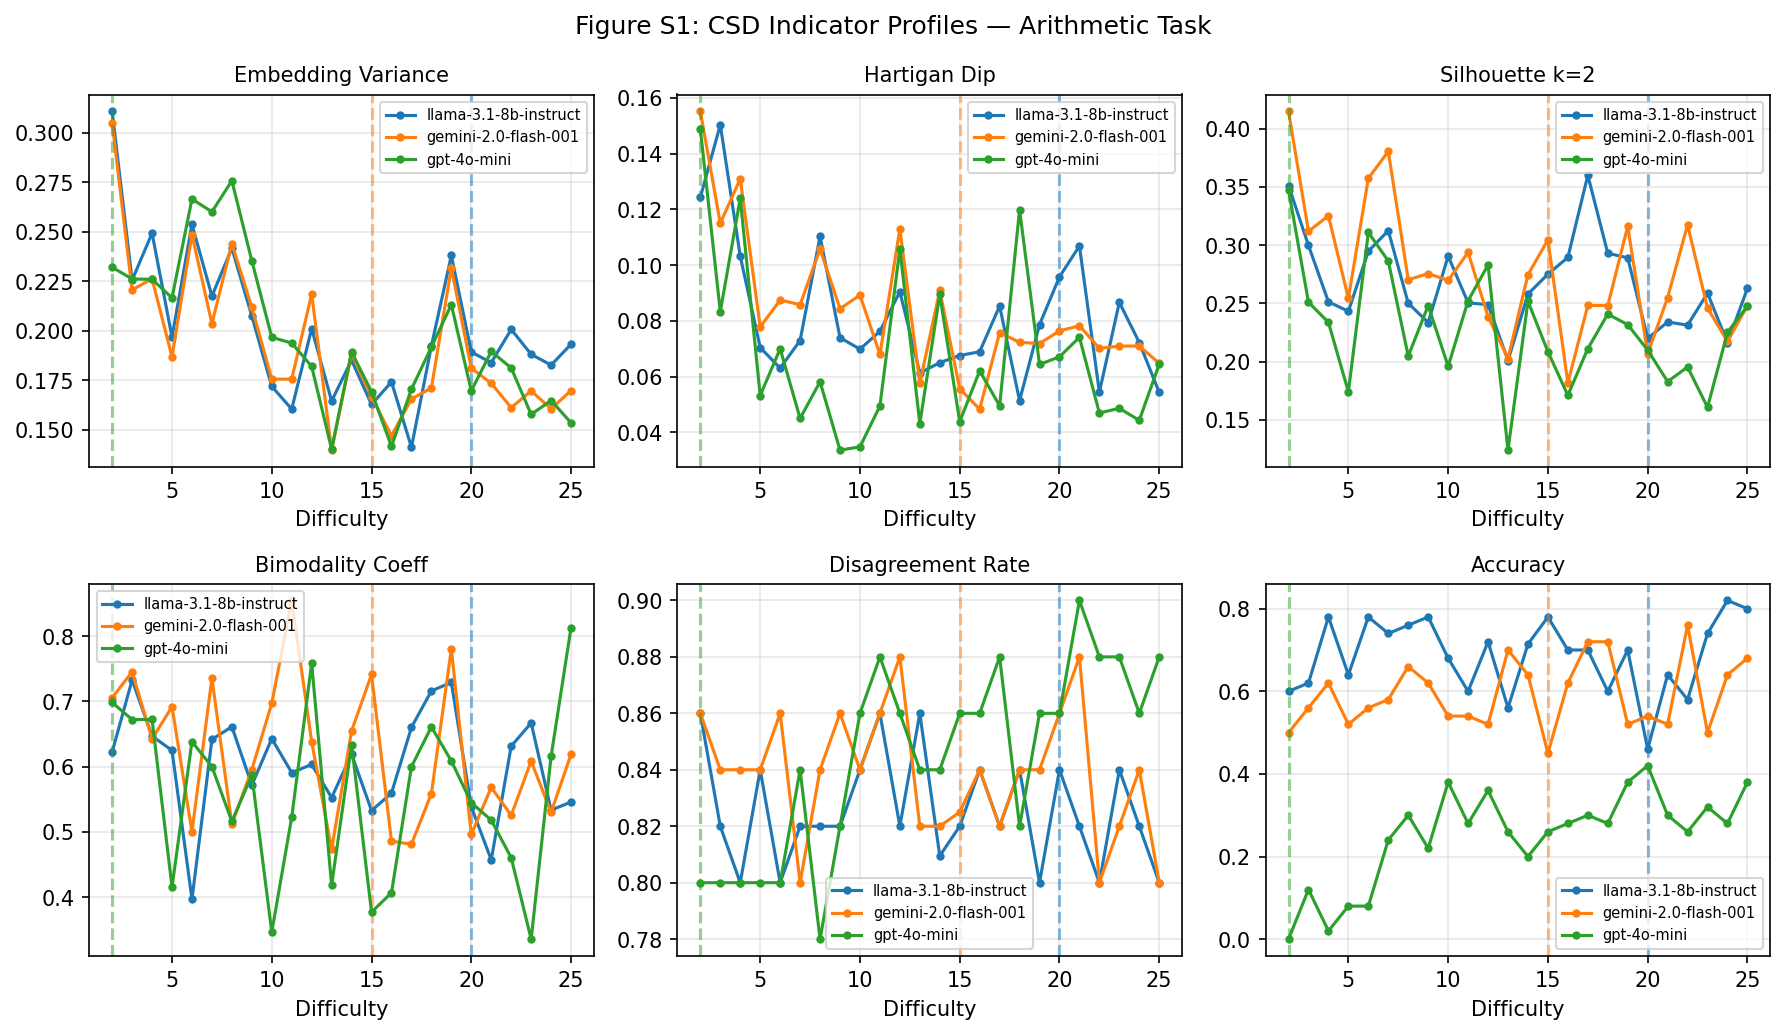
\includegraphics[width=0.9\textwidth]{figures/figure_s1.png}
\caption{CSD Indicator Profiles -- Arithmetic Task}
\end{figure}

\begin{figure}[h]
\centering
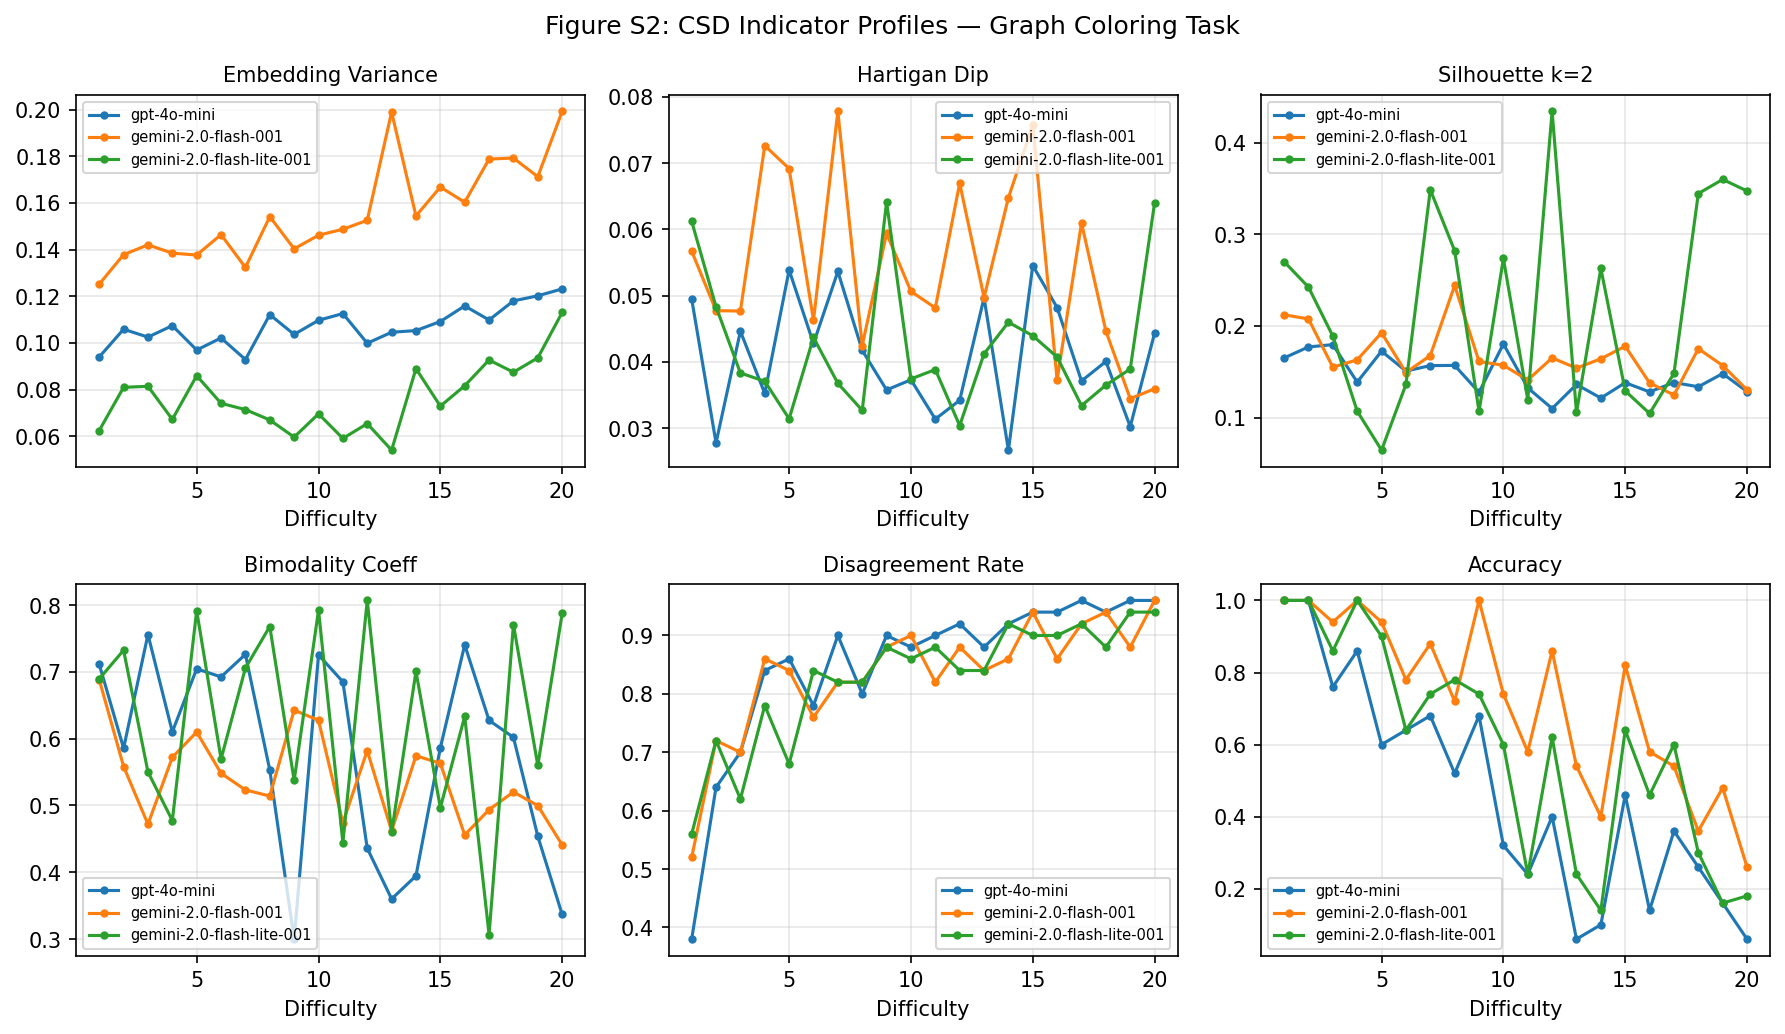
\includegraphics[width=0.9\textwidth]{figures/figure_s2.png}
\caption{CSD Indicator Profiles -- Graph Coloring Task}
\end{figure}

\begin{figure}[h]
\centering
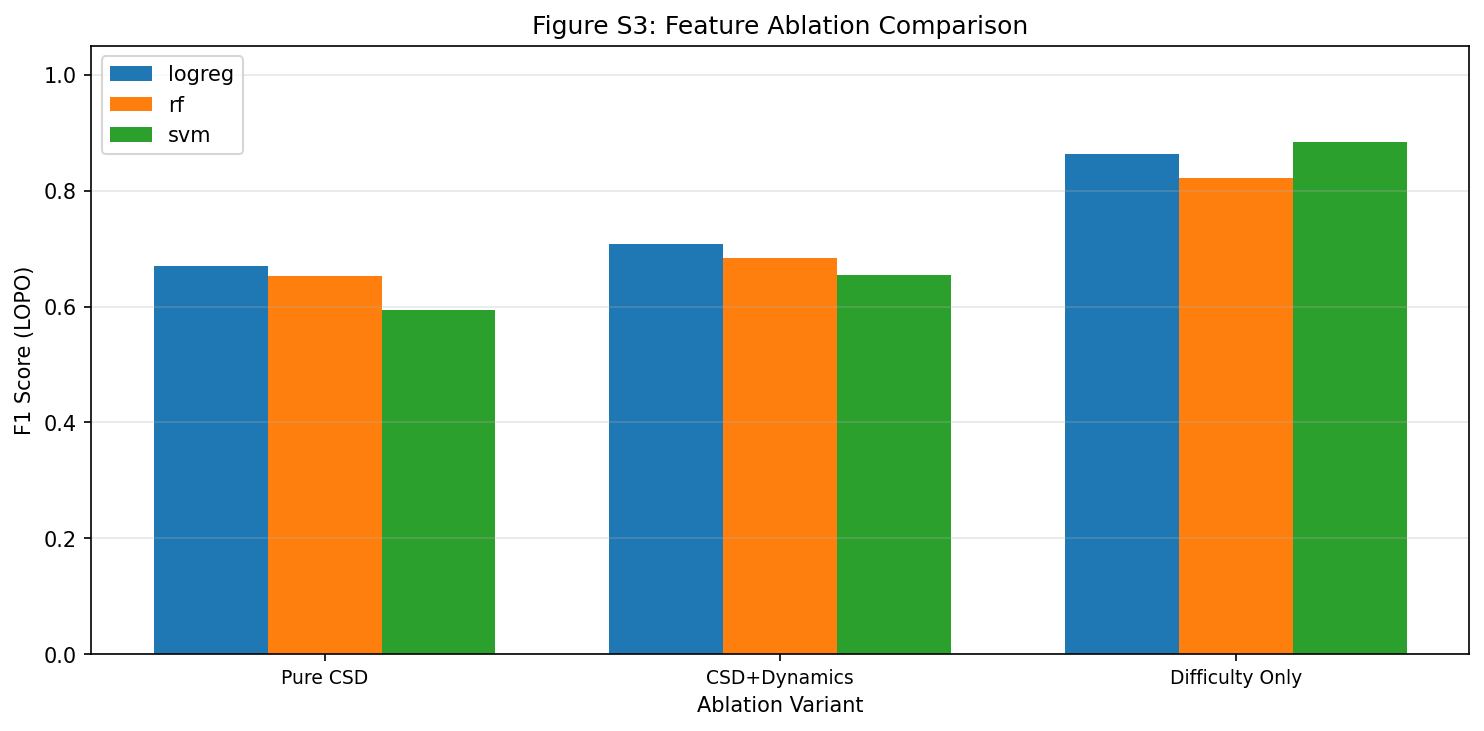
\includegraphics[width=0.9\textwidth]{figures/figure_s3.png}
\caption{Feature Ablation Comparison}
\end{figure}

\begin{figure}[h]
\centering
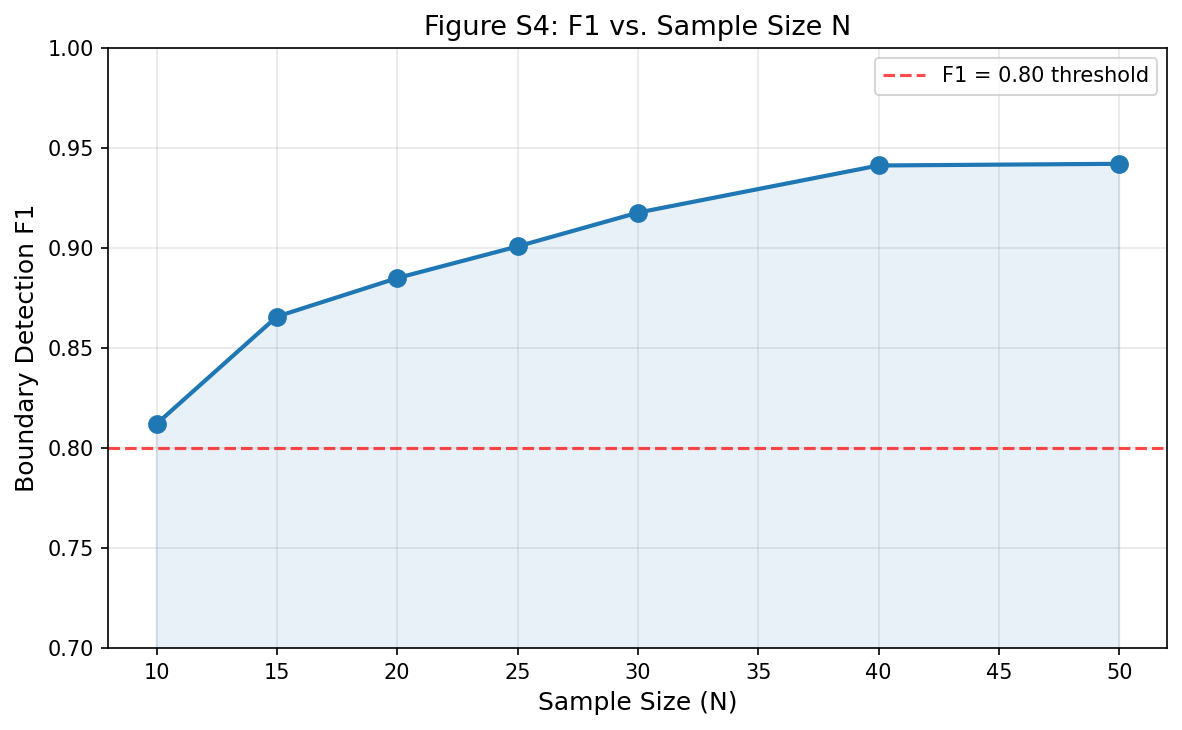
\includegraphics[width=0.9\textwidth]{figures/figure_s4.png}
\caption{F1 vs.\ Sample Size N}
\end{figure}


\end{document}
